\chapter{Dissertation or Thesis Format}
\label{ch:2}

The following guidelines offer you some degree of flexibility in formatting your thesis or dissertation.
Whichever options you choose to use, you must use them consistently throughout the document.

\section{Margins}

Your printed output must reflect physically measurable top, bottom, left, and right margins of 1 inch.
Some systems' settings produce varying results when printing to different printers, so be sure to measure your output.
Remember, nothing, not even page numbers, should print in the margins.

\section{Page Numbers}

All pages numbers should be placed on the center of each page immediately above the bottom margin.
Number all pages in your document except for the title page and the optional copyright page which might follow the title page.
Number the ``front matter'' pages (i.e., the pages that come prior to the main body of text, prior to chapter 1) with lowercase roman numerals, starting with ii (remember, the title page is counted but not numbered, and the copyright page is neither counted nor numbered).
The body of the dissertation or thesis should be numbered with Arabic numerals starting with 1 and should begin on the epigraph page (optional), the introduction, if one is used, or on the first page of the first chapter.
Options are summarized in Table~\ref{tab:include} on page two.

\section{Text}

This template uses a 12-point, Times New Roman font throughout and is recommended for your dissertation or thesis.
However, should you choose to use a different font, you should match the font size as close as possible.
Use double-spacing for body text.
Use either left justification with a ragged right edge or full justification.

\section{Chapter Titles}

Begin each chapter on a new page.
You may start the chapter title below the top margin or you may leave some space and start the chapter title up to 3 inches from the top edge of the page.
The font size for chapter titles should be no larger than 24.
There are two options for formatting the chapter title:

\begin{enumerate}
	\item Type the word ``Chapter'' followed by the chapter number, skip a line, and type the chapter title on the following line; or
	\item Type the chapter number followed by the chapter title, all on the same line.
\end{enumerate}

\section{Section Headings \& Numbering}

Headings may be typed above or on the same line as the sections they label.
Type the chapter number and section number before the section title.
The font size for section headings should be no larger than 18.

\subsection{Subsection Headings \& Numbering}
\label{subsec:subsection-headings-numbering}

This should follow the usual convention of your discipline and be acceptable to your committee; if your discipline calls for them they must be in included in the table of contents.
Type the chapter number, section number and subsection number before the subsection title.
The font size for subsection headings should be no larger than 14.

\subsubsection{Headings for Divisions Smaller than Subsections}

Do not number headings for divisions smaller than subsections.
These are not included in the table of contents.
Headings may be typed above or on the same line as the sections they label.
Divisions smaller than subsections should be the same font size as the body text.

\section{Figures and Tables}

There are two options for numbering your figures and tables; choose one and be consistent in its use throughout your document.
In either case, the name and description of the figure or table should be single spaced and can be a smaller font size.

\begin{enumerate}
	\item Maintain a separate numbering sequence for your list of figures and list of tables.
Label figures with the word ``Figure'' and tables with the word ``Table''; or
	\item Label both figures and tables with the word ``Figure'' and maintain one numbering sequence.
\end{enumerate}

Place figures and tables as close to their reference in the text as possible.
Do not let figures or tables spill out into the margins.

\begin{enumerate}
	\item Place the figure number and title below each figure (or table labeled as a figure).
	\item Place the table number and title above each table labeled as a table.
\end{enumerate}

\begin{figure}
  
\includegraphics{figures/just-a-figure}
  \caption[Left justified figure]{You can left justify your figure.}
  \label{fig:left-justified}
\end{figure}

\begin{figure}
  \centering
  
\includegraphics{figures/just-a-figure}
  \caption[Centered figure]{You can center your figure.}
  \label{fig:centered}
\end{figure}

This \LaTeX template is configured to produce a PDF.
Your figures should be PDF files like Figure~\ref{fig:pdf}.
If you do not have a PDF version of your figure, \emph{latexmk} and \emph{emph} can convert the image to PDF for you as shown in Figure~\ref{fig:svg}.

\begin{figure}
  \centering
  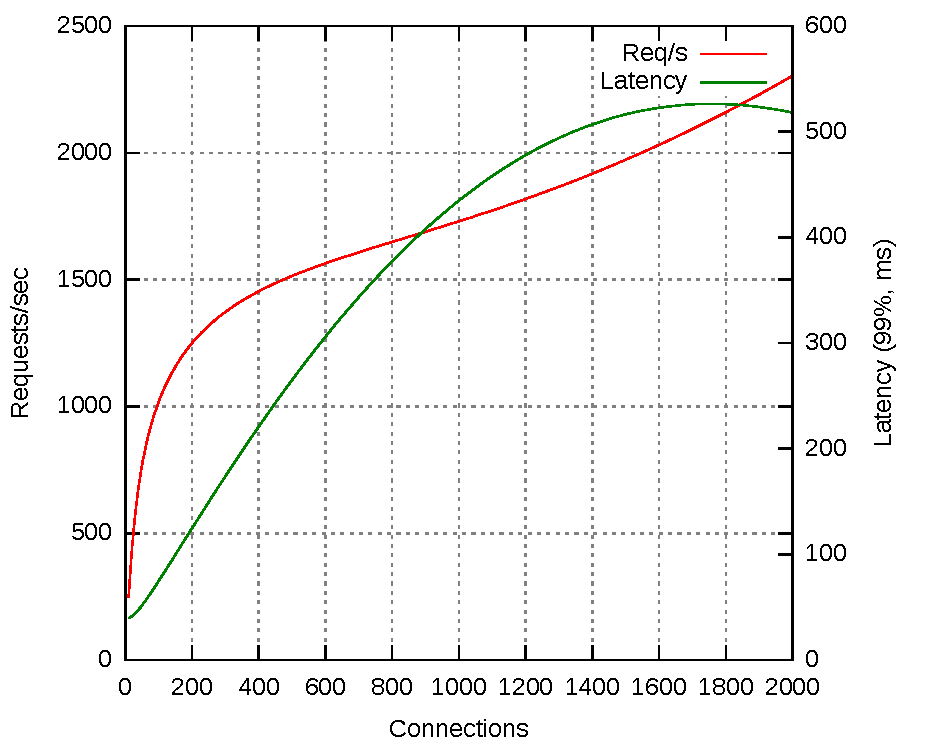
\includegraphics{figures/just-a-plot}
  \caption[Figures must be PDF]{All figures must be PDFs.}
  \label{fig:pdf}
\end{figure}

\begin{figure}
  \centering
  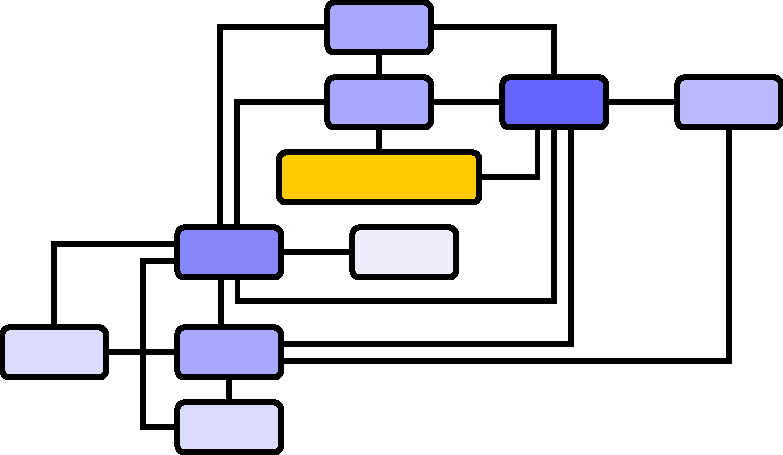
\includegraphics{figures/just-a-graph}
  \caption[SVG converted to PDF]{the \texttt{Makefile} and \texttt{latexmkrc} files include a rule to convert SVG images to PDF images.
	\emph{latexmk} will convert EPS files for you too.}
  \label{fig:svg}
\end{figure}

\section{Lists}

You may include lettered, numbered, or bulleted lists in your document.
Use consistent punctuation and capitalization throughout each list.
Lists may be indented.

\section{Footnotes and Endnotes}

You may use footnotes or endnotes for brief notes that are not appropriate for the body of the text.\footnote{The use of endnotes and footnotes should follow the usual convention of your discipline and be acceptable to your committee.}
Use either footnotes or endnotes consistently throughout your dissertation or thesis.
Endnotes are positioned at the end of each chapter.
Single-space within each footnote or endnote.
Footnotes should be numbered consecutively within a chapter; numbers should restart with each new chapter.
Endnotes should be numbered consecutively through the entire body of your dissertation or thesis.

\section{Quotations}

You must use quotation marks and parenthetical references to indicate words that are not your own.
Put quotation marks around short quotes.
Put long quotes in separate single-spaced paragraphs, indented up to 1 inch from the left margin (these are called block quotations).
Kate Turabian, editor of official publications and dissertation secretary at the University of Chicago for over 25 years, distinguishes short and long quotes as follows:

\begin{quote}
    Short, direct prose quotations should be incorporated into the text of the paper and enclosed in
    double quotation marks: ``One small step for man; one giant leap for mankind.'' But in general a
    prose quotation of two or more sentences which at the same time runs to four or more lines of
    text in a paper should be set off from the text and indented in its
    entirety\ldots~\cite{Turabian}
\end{quote}

\section{Equations}

Equation numbering and formatting should follow the usual convention of your discipline and be acceptable to your committee.

Equations may be set in-line with the text or numbered and placed in separate paragraphs.
Use the same numbering style for equations as you would for figures and tables.
Here is an example of an equation set in-line with a paragraph: $E = mc^{2}$.
Here is an example equation placed in a separate paragraph:

\begin{align}
	E = mc^{2}
\end{align}
